\chapter{TP1 --- TCP Communication Between Client Processes and a Server Process}

% -----------------------------------------------------------------------
\section{Objectives}

The goal of this lab is to establish a TCP client-server architecture in Java. The server stores a university library catalog in memory, processes client requests sequentially (without multithreading), and responds to read-only queries.

% -----------------------------------------------------------------------
\section{Exercise 1 --- Identification and Local Implementation}

\subsection{Architecture Analysis}

The system consists of four primary components:
\begin{itemize}[leftmargin=*]
  \item \textbf{Client (\texttt{ClientBibliotheque}):} Prompt user input (\texttt{LISTE} or \texttt{RECHERCHE;theme}), send TCP requests, receive and display responses without executing business logic.
  \item \textbf{Server (\texttt{ServeurBibliotheque}):} Listen for TCP connections, delegate parsing to \texttt{ProtocoleBibliotheque} and execution to \texttt{GestionBibliotheque}, then return results.
  \item \textbf{Service:} Provide two features: displaying all catalog books and searching books by topic.
  \item \textbf{Service Interface:} Define operations \texttt{listerLivres()} and \texttt{rechercherParTheme(String theme)}, including validation rules (\texttt{IllegalArgumentException} on blank/null topics).
\end{itemize}

\subsection{Service Interface Contract}

The functional contract guarantees:
\begin{itemize}[leftmargin=*]
  \item \texttt{listerLivres()}: Returns all catalog books in their original order.
  \item \texttt{rechercherParTheme(theme)}: Returns matching books via case-insensitive full-topic comparison, ignoring leading/trailing spaces. Throws an \texttt{IllegalArgumentException} for \texttt{null}, empty, or whitespace-only inputs.
\end{itemize}

\subsection{Implementation Overview}

\begin{itemize}[leftmargin=*]
  \item \textbf{Domain Classes (\texttt{Livre}, \texttt{Bibliotheque}):} Model book attributes (ID, title, topics) with normalized comparisons, and initialize the default 5-book catalog (\texttt{L1}--\texttt{L5}).
  \item \textbf{Business Logic (\texttt{GestionBibliotheque}):} Pure domain service executing queries without socket or network dependencies.
\end{itemize}

\begin{figure}[htbp]
  \centering
  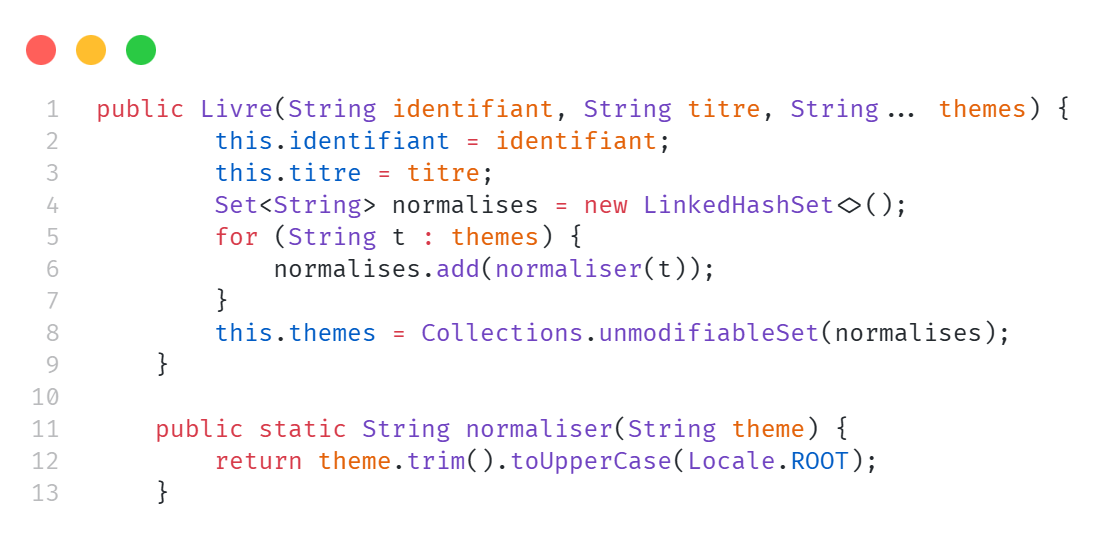
\includegraphics[width=0.9\textwidth]{Figures/Livre_Constructor.png}
  \caption{\texttt{Livre} Class Initialization}
  \label{fig:livre-constructor}
\end{figure}

\begin{figure}[htbp]
  \centering
  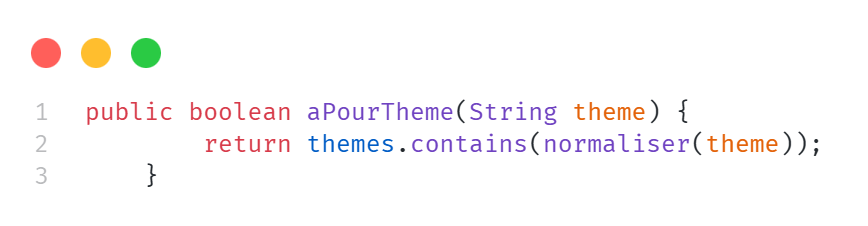
\includegraphics[width=0.9\textwidth]{Figures/Livre_Constructor_Theme.png}
  \caption{\texttt{Livre} Theme Normalization and Verification}
  \label{fig:livre-theme}
\end{figure}

\begin{figure}[htbp]
  \centering
  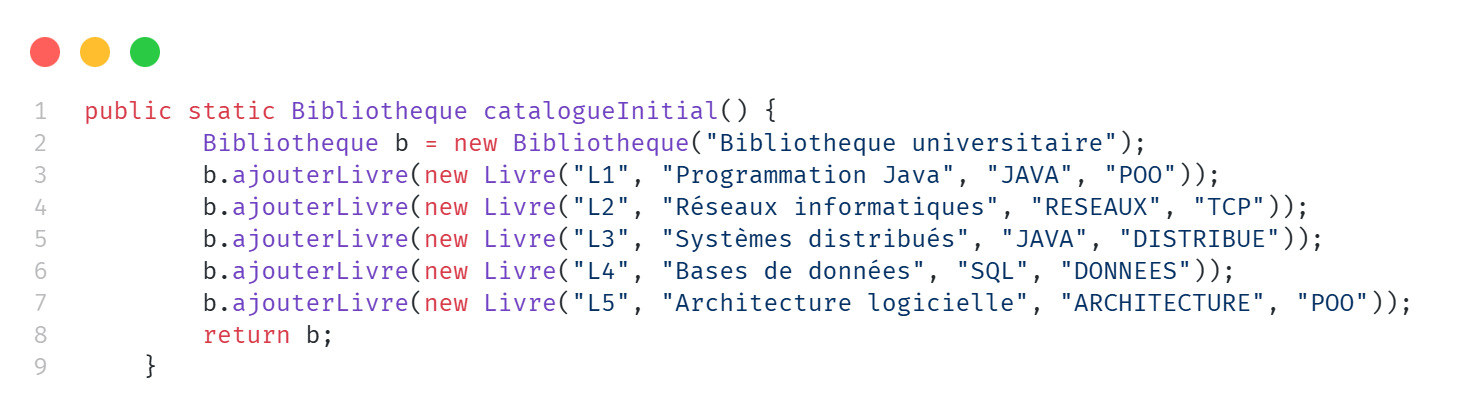
\includegraphics[width=0.9\textwidth]{Figures/Biblio_catalogueInitial.png}
  \caption{Initial Catalog Setup in \texttt{Bibliotheque}}
  \label{fig:biblio-catalog}
\end{figure}

\begin{figure}[htbp]
  \centering
  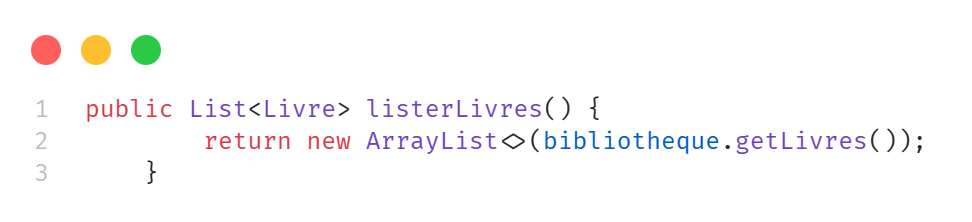
\includegraphics[width=0.9\textwidth]{Figures/listerLibres.png}
  \caption{Implementation of \texttt{listerLivres()} in \texttt{GestionBibliotheque}}
  \label{fig:lister-livres}
\end{figure}

\begin{figure}[htbp]
  \centering
  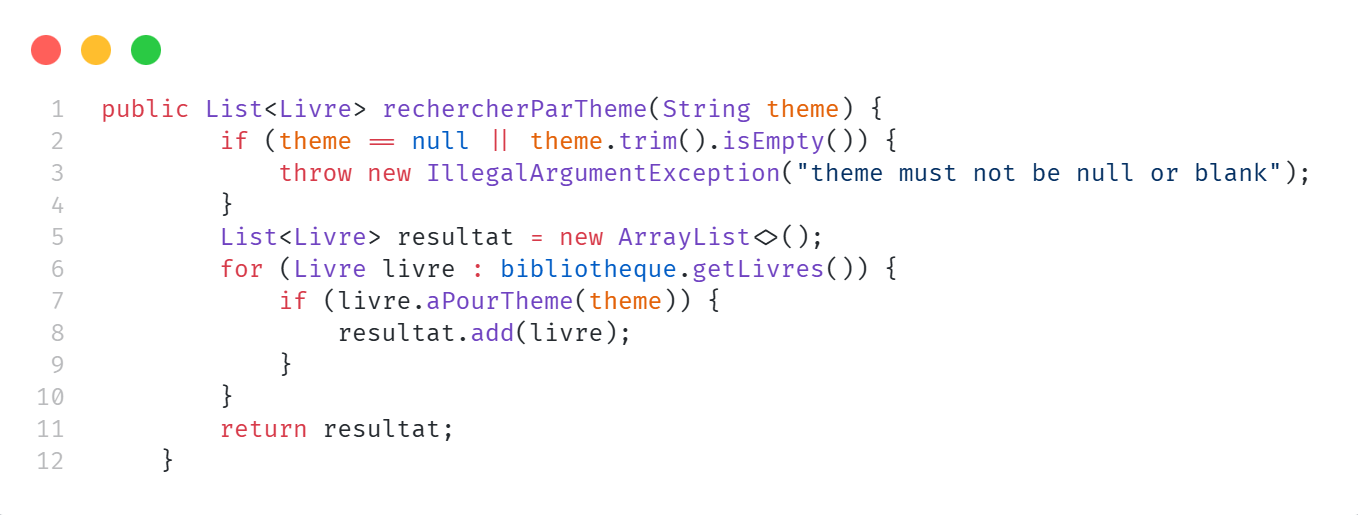
\includegraphics[width=0.9\textwidth]{Figures/rechercher_par_theme.png}
  \caption{Implementation of \texttt{rechercherParTheme()} in \texttt{GestionBibliotheque}}
  \label{fig:rechercher-theme}
\end{figure}

\subsection{Local Validation}

Local unit tests (\texttt{TestBibliothequeLocal}) confirmed all core features, including full catalog listing, topic search filtering, case-insensitivity, and exception handling for invalid inputs.

\begin{figure}[htbp]
  \centering
  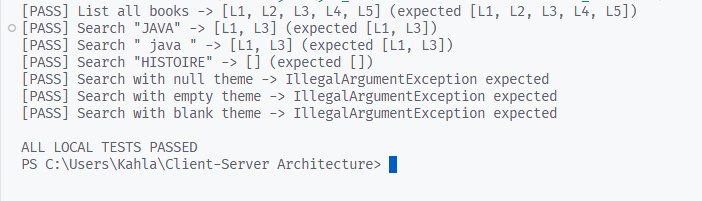
\includegraphics[width=0.9\textwidth]{Figures/test_local_results.png}
  \caption{Local Unit Test Execution Results}
  \label{fig:test-local}
\end{figure}

\medskip
\textbf{Question:} Connecting separate processes requires replacing direct local Java method calls with TCP socket message exchanges.

% -----------------------------------------------------------------------
\section{Exercise 2 --- First TCP Communication (PING/PONG)}

\subsection{Communication Mechanism}

The server uses \texttt{ServerSocket.accept()} to receive client connections, while the client initiates a connection via \texttt{Socket(host, port)}. Messages are exchanged line-by-line in UTF-8 over \texttt{BufferedReader}/\texttt{BufferedWriter} streams, finalized with \texttt{flush()}.

\subsection{Execution Results}

Running client and server as distinct processes over \texttt{127.0.0.1:5000} successfully returns \texttt{PONG} for a \texttt{PING} request, and \texttt{ERR;COMMANDE\_INCONNUE} otherwise. Disconnecting the server triggers a connection failure alert on the client. 

\begin{figure}[htbp]
  \centering
  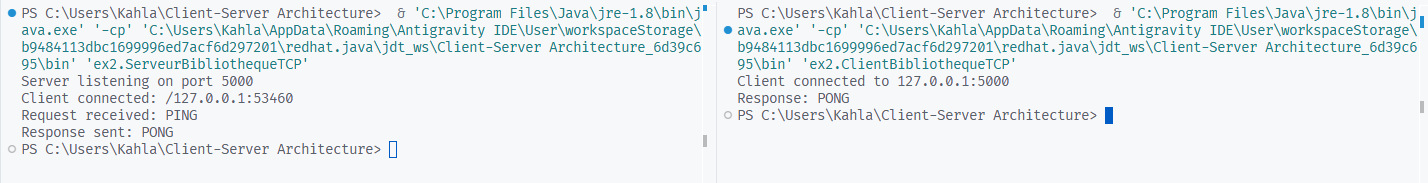
\includegraphics[width=0.9\textwidth]{Figures/ping_pong_execution.png}
  \caption{PING/PONG Console Execution Output}
  \label{fig:ping-pong}
\end{figure}

% -----------------------------------------------------------------------
\section{Exercise 3 --- Library Services over TCP}

\subsection{Protocol Mapping}

Requests map directly to protocol lines: \texttt{LISTE} retrieves all books, and \texttt{RECHERCHE;theme} searches by topic. Successful responses follow \texttt{OK;n;id:title;...} (or \texttt{OK;0} when empty). Protocol errors yield \texttt{ERR;COMMANDE\_INCONNUE} or \texttt{ERR;REQUETE\_INVALIDE}. Reserved delimiting characters (\texttt{;}, \texttt{:}, \texttt{,}) in search topics render requests invalid.

\subsection{Architecture Setup}

\begin{itemize}[leftmargin=*]
  \item \textbf{\texttt{ProtocoleBibliotheque}:} Decouples network communication from business logic by parsing line requests and formatting response strings.
  \item \textbf{\texttt{ServeurBibliotheque}:} Runs an infinite loop serving client requests sequentially with a 10-second socket timeout.
  \item \textbf{\texttt{ClientBibliotheque}:} Configurable client connecting to target IP/port, sending formatted commands, and printing responses.
\end{itemize}

\begin{figure}[htbp]
  \centering
  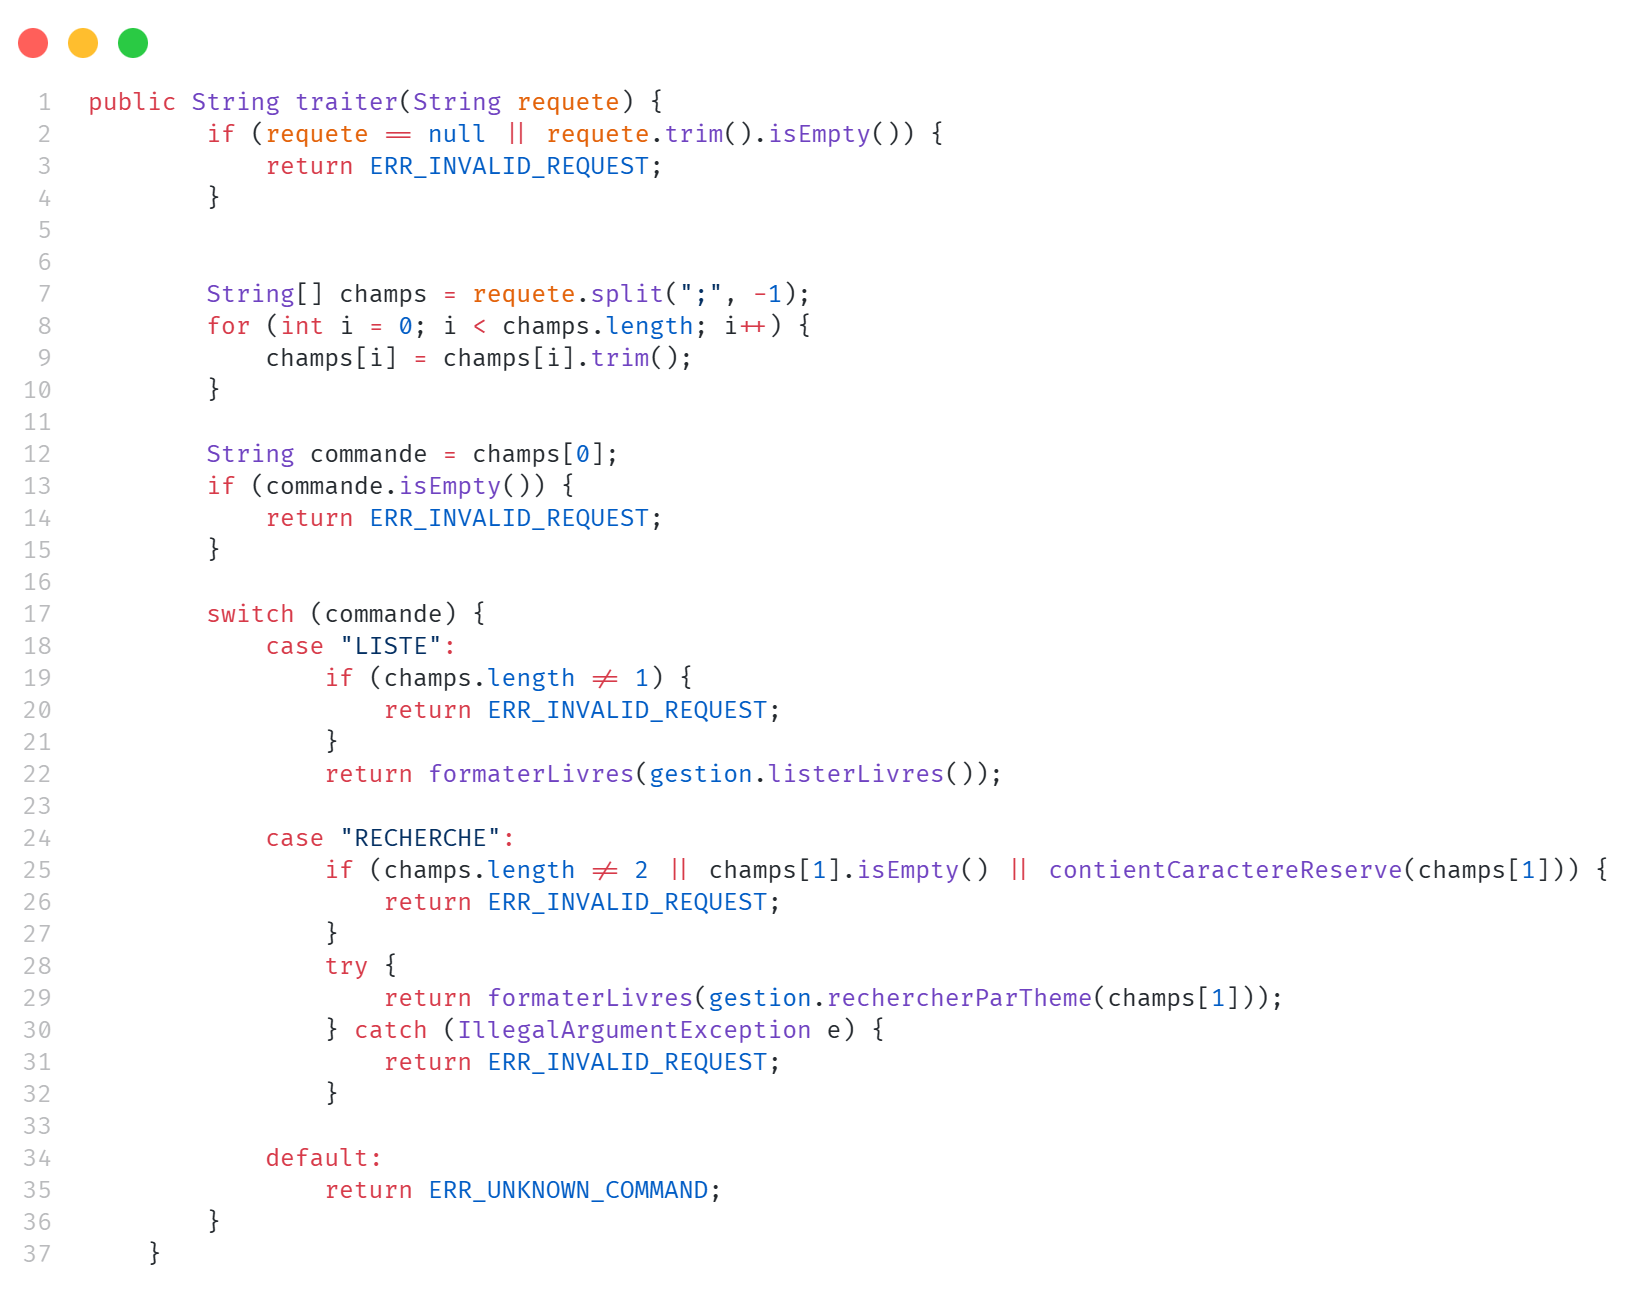
\includegraphics[width=0.9\textwidth]{Figures/ex3_server_code.png}
  \caption{Protocol and Server Implementation Details}
  \label{fig:ex3-server-code}
\end{figure}

\subsection{\texorpdfstring{Validation \& Testing}{Validation and Testing}}

All scenario test cases passed successfully: querying all books (\texttt{LISTE}), searching valid topics (\texttt{RECHERCHE;JAVA}), handling empty results (\texttt{RECHERCHE;HISTOIRE}), invalid syntax errors, robust server recovery after client errors, and remote deployment across distinct network hosts.

\begin{figure}[htbp]
  \centering
  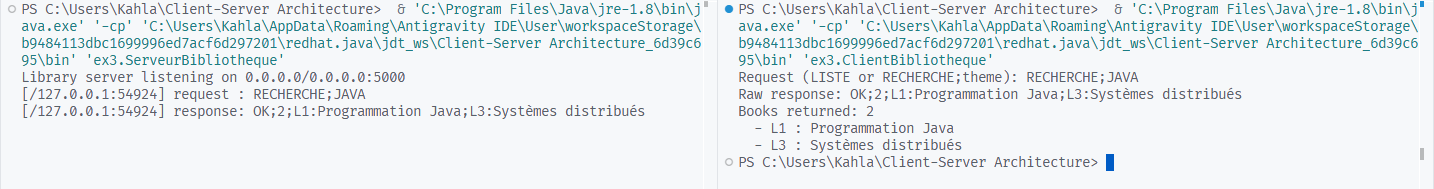
\includegraphics[width=0.9\textwidth]{Figures/exercise3_execution.png}
  \caption{Exercise 3 Service Execution Outputs}
  \label{fig:ex3-execution}
\end{figure}

% -----------------------------------------------------------------------
\section{\texorpdfstring{Synthesis \& Questions}{Synthesis and Questions}}

\subsection{Final System Structure}

\begin{itemize}[leftmargin=*]
  \item \textbf{Client:} \texttt{ClientBibliotheque} (Client Process) --- Handles user input/output and TCP communication.
  \item \textbf{Server:} \texttt{ServeurBibliotheque} \& \texttt{ProtocoleBibliotheque} (Server Process) --- Handles socket listening, request parsing, and protocol formatting.
  \item \textbf{Service:} \texttt{GestionBibliotheque} (Server Process) --- Executes domain catalog queries.
  \item \textbf{Interface:} \texttt{GestionBibliotheque} signatures + TCP protocol specification --- Defines the functional and operational contract.
\end{itemize}

\subsection{Q1 --- Service, Interface, and Protocol}

\begin{itemize}[leftmargin=*]
  \item \textbf{Service Operation:} The business logic processing executed by \texttt{GestionBibliotheque.rechercherParTheme}.
  \item \textbf{Interface (Contract):} Transport-independent signature and behavior rules (non-empty topic parameter, catalog order, throwing \texttt{IllegalArgumentException}).
  \item \textbf{Protocol:} Network message representation handled by \texttt{ProtocoleBibliotheque} (\texttt{RECHERCHE;theme} $\rightarrow$ \texttt{OK;n;...} or \texttt{ERR;...}).
\end{itemize}

\subsection{Q2 --- Direct Objects vs. TCP Requests}

Client and server execute in separate operating system memory spaces (often on distinct network nodes). Direct Java method calls cannot cross process boundaries, requiring data to be serialized as text messages transmitted over TCP.

\subsection{Q3 --- Evolution Toward Middleware}

\begin{itemize}[leftmargin=*]
  \item \textbf{To Retain:} Domain logic (\texttt{GestionBibliotheque}), data models (\texttt{Livre}, \texttt{Bibliotheque}), and functional contract signatures.
  \item \textbf{To Replace:} Manual network plumbing (sockets, stream readers/writers, custom parsing in \texttt{ProtocoleBibliotheque}) is completely replaced by middleware stubs and skeletons (e.g., RMI).
\end{itemize}